\section{Расчет биологической защиты} %TODO: убрать для репорта
\subsection{Постановка задачи}
Необходимо рассчитать дозу облучения при стационарном режиме работы ЯЭУ ВВЭР-1000 за биологической защитой

\subsection{Построение расчетной модели биологической защиты}
Для формирования расчетной модели рассмотрим компоновку элементов и помещений ЯЭУ с РУ ВВЭР-1000.

\begin{figure}[H]
	\begin{center}
		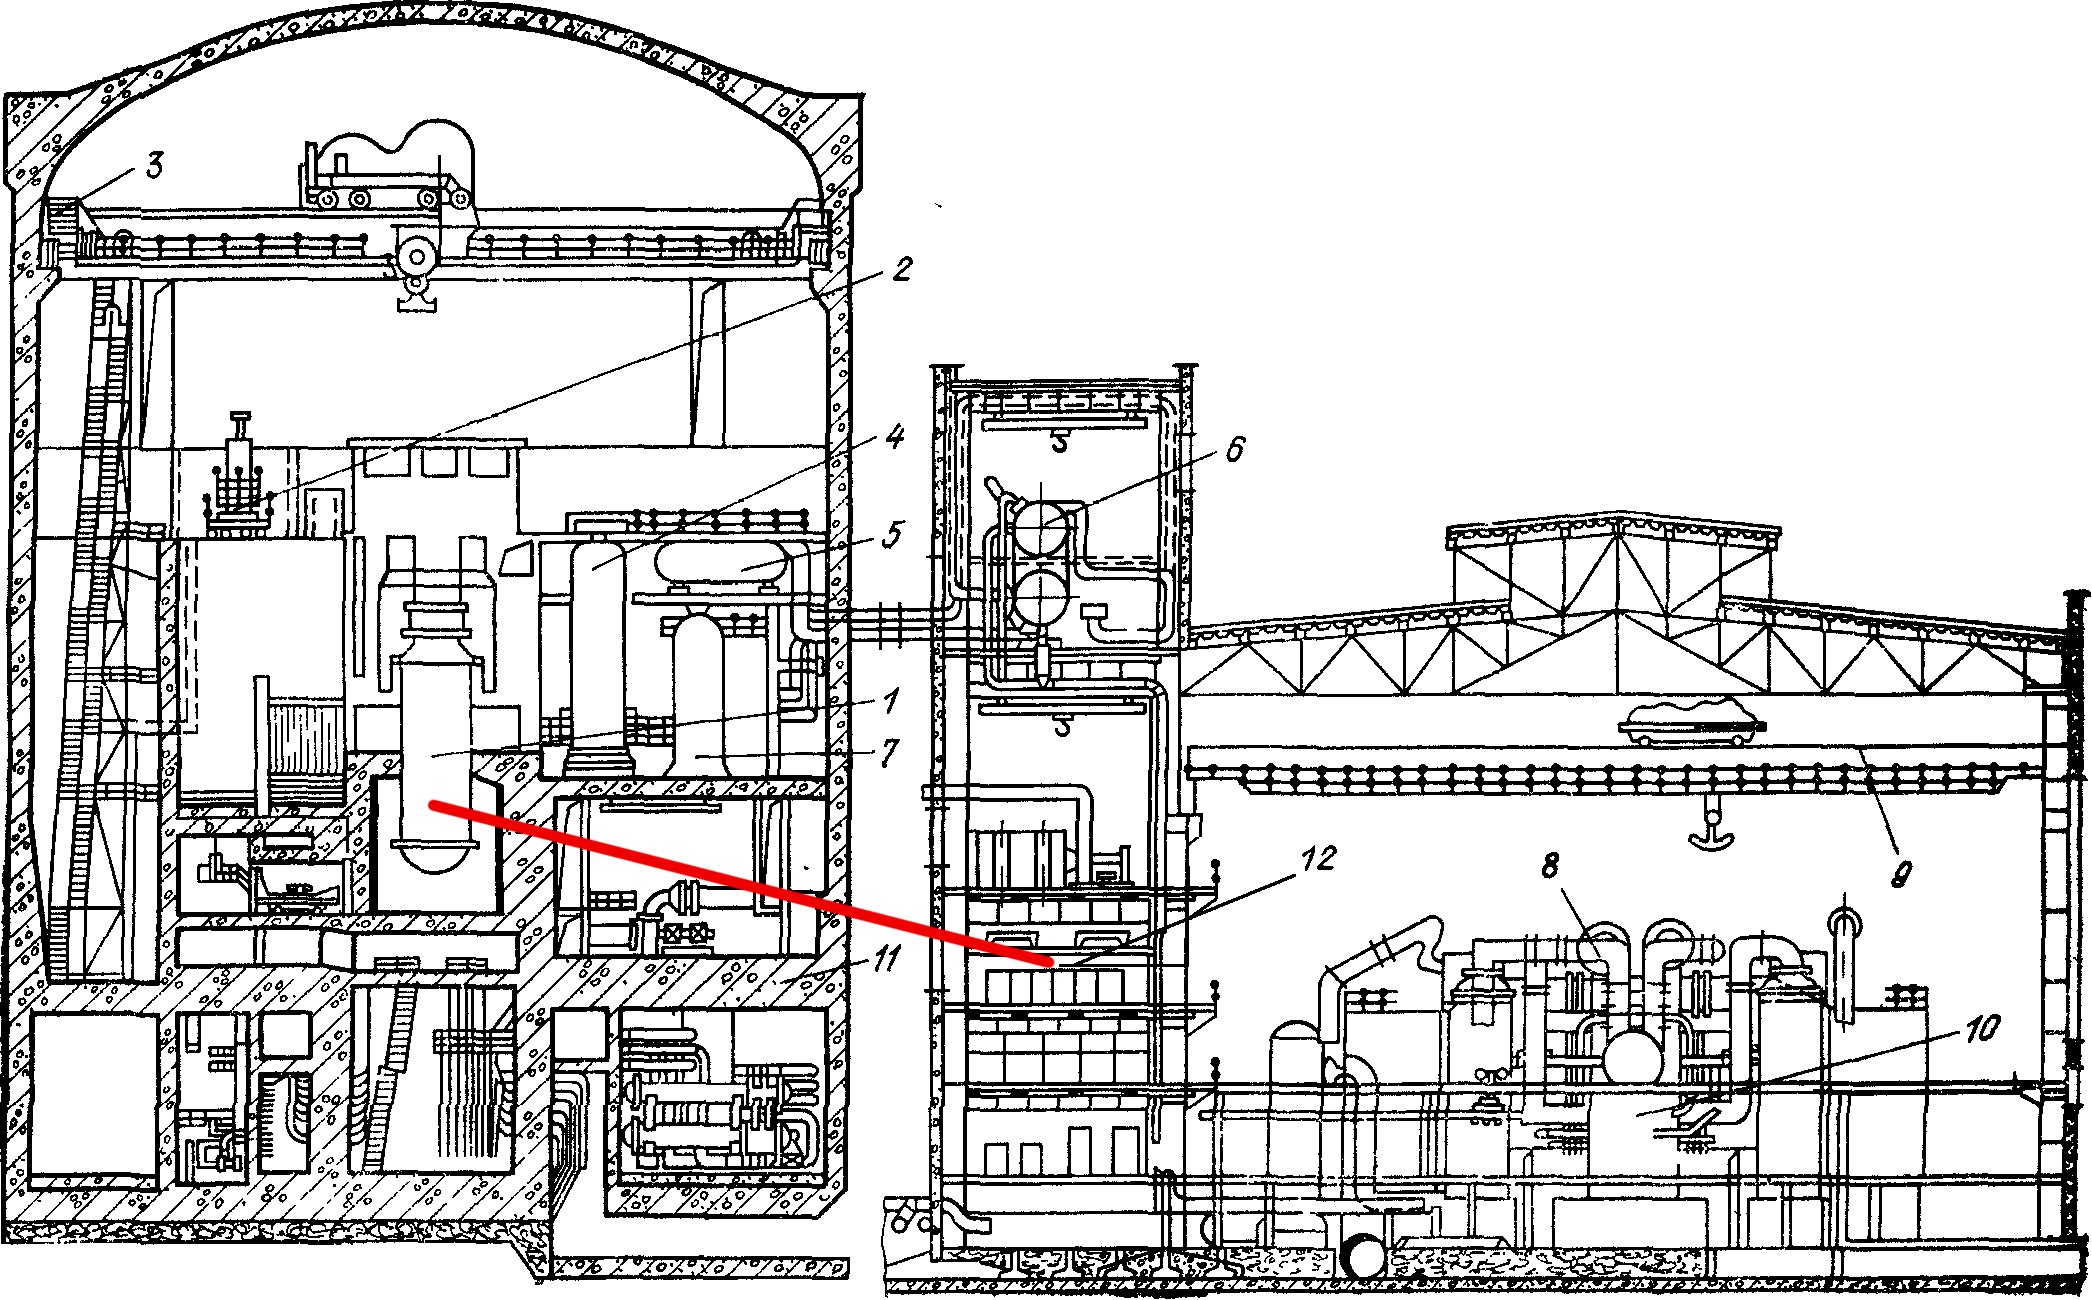
\includegraphics{razrez_bio.png}
		\caption{Компоновка энергоблока с РУ ВВЭР-1000 (Южно-Украинская АЭС)}
		\label{pic:razrez_bio} % название для ссылок внутри кода
	\end{center}
\end{figure}
% Монахов Атомные электрические станции и их технологическое оборудование
